%
	\section{Oxygen Plasma Chemistry}\label{sec:negionphysics}
%
		In comparison to most inert working gases in ccrf discharges, oxygen has an overwhelming number of reaction sets for collisions of elastic, inelastic and reactive character. Additionally, the negative ion species has to be taken into account when discussing collisional processes. For example, an in-depth benchmarking of both simulated and experimentally measured cross section data is given by Gudmundsson et al.\@ in~\cite{Gudmundsson13}. There, 33 collisions and reactions have been revisited, already reducing the investigation to the most important processes in ccrf plasma. In this thesis the selection of possible reactions will be based on~\cite{Bronold07b} and slightly modified. The final collection of cross sections can be found in~\autoref{tab:cross_sections} and observed in~\autoref{fig:cross_sections_mine}. Those data are semi-empirical, meaning part of them are based on measurements in finite energy ranges and low-/high-energy asymptotic models. Cross sections for very high energies are not important, as the collision probability usually decays very fast here.\\
		As already seen in~\autoref{sec:heating}, collisions strongly influence the particle distribution functions and density profiles. Furthermore, a good understanding of the plasma chemistry is key to, e.g.\@ applications in surface physics supported by gas discharges. Of high importance for plasma-assisted material processes is the generation of negative ions. Hence the ratio $\alpha=n\ix{i,-}/n\ix{e}$ is important to characterize the electronegative plasma, like a ccrf oxygen discharge by $\alpha>1$.\\
		I will highlight the most important collisions and reactions in the following section. 
%
		\begin{longtable}{lll}
			\toprule%
				\bfseries Nr. & \bfseries Reaction & \bfseries Type \\%
			\toprule\midrule\endhead%
						& \bfseries Elastic scattering 							& \bfseries Energy loss 	\\% 
						$(1)$  & $e^{-}+O\ix{2}			 	\rightarrow	O\ix{2}+e^{-}$ &						\\%
						$(2)$  & $O^{-}+O\ix{2}			 	\rightarrow	O\ix{2}+O^{-}$ & 						\\%
						$(3)$  & $O\ix{2}^{-}+O\ix{2} \rightarrow	O\ix{2}+O\ix{2}^{-}$ & 			\\ \midrule%
						& \bfseries Electron energy loss scattering & \bfseries Energy loss 	\\%
						$(4)$  & $e^{-}+O\ix{2}			 	\rightarrow	O\ix{2}^{\nu}+e^{-}$ & %
										Vibrational excitation	($\nu=1,\dots,4$)											\\%
						$(5)$  & $e^{-}+O\ix{2}			 	\rightarrow	O\ix{2}(Ryd)+e^{-}$ & %
										Rydberg excitation																						\\%
						$(6)$  & $e^{-}+O\ix{2}			 	\rightarrow	O(1D)+O(3P)+e^{-}$ & %
										Dissociative excitation at $\unit[8,6]{eV}$										\\%
						$(7)$  & $e^{-}+O\ix{2}		 	 	\rightarrow	O\ix{2}%
																					 (a^{1}\Delta\ix{g},b^{1}\Sigma\ix{g})$ & %
										Meta-stable excitaion																					\\ \midrule%
						& \bfseries Electron and ion reactions & \bfseries Creation and loss 	\\%
						$(8)$  & $e^{-}+O\ix{2}^{+}	 	\rightarrow	2\,O$ & %
										Dissociative recombination 																		\\%
						$(9)$  & $O^{-}+O\ix{2}^{+}	 	\rightarrow	O\ix{2}+O$ & %
										Neutralization						 																		\\%
						$(10)$ & $e^{-}+O\ix{2}	 		 	\rightarrow	O+O^{-}$ & %
										Dissociative attachment		 																		\\%
						$(11)$ & $O^{-}+O\ix{2}			 	\rightarrow	O+O\ix{2}+e$ & %
										Direct detachment 																						\\%
						$(12)$ & $e^{-}+O\ix{2}		 		\rightarrow	2e^{-}+O\ix{2}^{+}$ & %
										Impact ionization 																						\\%
						$(13)$ & $e^{-}+O^{-}			 		\rightarrow	O+2e^{-}$ & %
										Impact detachment																							\\%
			\midrule\bottomrule%
			\caption{%
				Most important colilision and reactions in ccrf plasma with the largest cross sections. %
				Empirical and simulated data, which have been included in this simulation are shown in~\autoref{fig:cross_sections}.}\label{tab:cross_sections}	
		\end{longtable}	
%		
		\subsection{Collisions and Reactions}\label{sec:negiondynamics}
%	
			The elastic collisions of $(1)--(3)$ conserve the particle numbers. Those are inter-species scattering processes, which will be assumed to have an isotropic inincident angle dependency~\cite{Bronold07b}. Intra-species elastic collisions were not very important at the selected parameter regions, though ion-ion scattering can strongly incluence the IEDF structure of the concerned densities are very high. However, for the electron species a binary \emph{coulomb scattering} process was used: the scattering angle $\chi$ is given by~\autoref{equ:coulomb_scatter} with $v\ix{rel}$ the relative velocity, $\ln\Gamma$ the Coulomb logarithm (see~\autoref{tabe:physicalquantities}) and $\tau\ix{c}$ the collision time.
%
			\begin{align}
				\langle\tan^{2}\frac{\chi}{2}\rangle=\frac{e^{4}n\ix{e}\ln\Gamma}%
					{8\pi\varepsilon\ix{0}m\ix{e}^{2}v\ix{rel}^{3}}\tau\ix{c}%
				\label{equ:coulomb_scatt}	
			\end{align}	
%
			The~\autoref{fig:cross_sections} shows the corresponding cross sections. In fact, only two are elastic processes, where as the collision of $O\ix{2}^{+}$ and the neutral molecule is a charge exchange reaction with momentum transfer. This kind of process:
%
			\begin{align}
				A^{-/+}+B\rightarrow A+B^{+/-}%
				\label{equ:charge_exchange}
			\end{align}
%
			is important for the consideration of surface effects. An ion with greater than thermal velocity coming from the wall will be cooled down by charge exchange collisions, which will transfer heat into the neutral reservior.\\

%			
			\begin{figure}[!b]
				\centering
				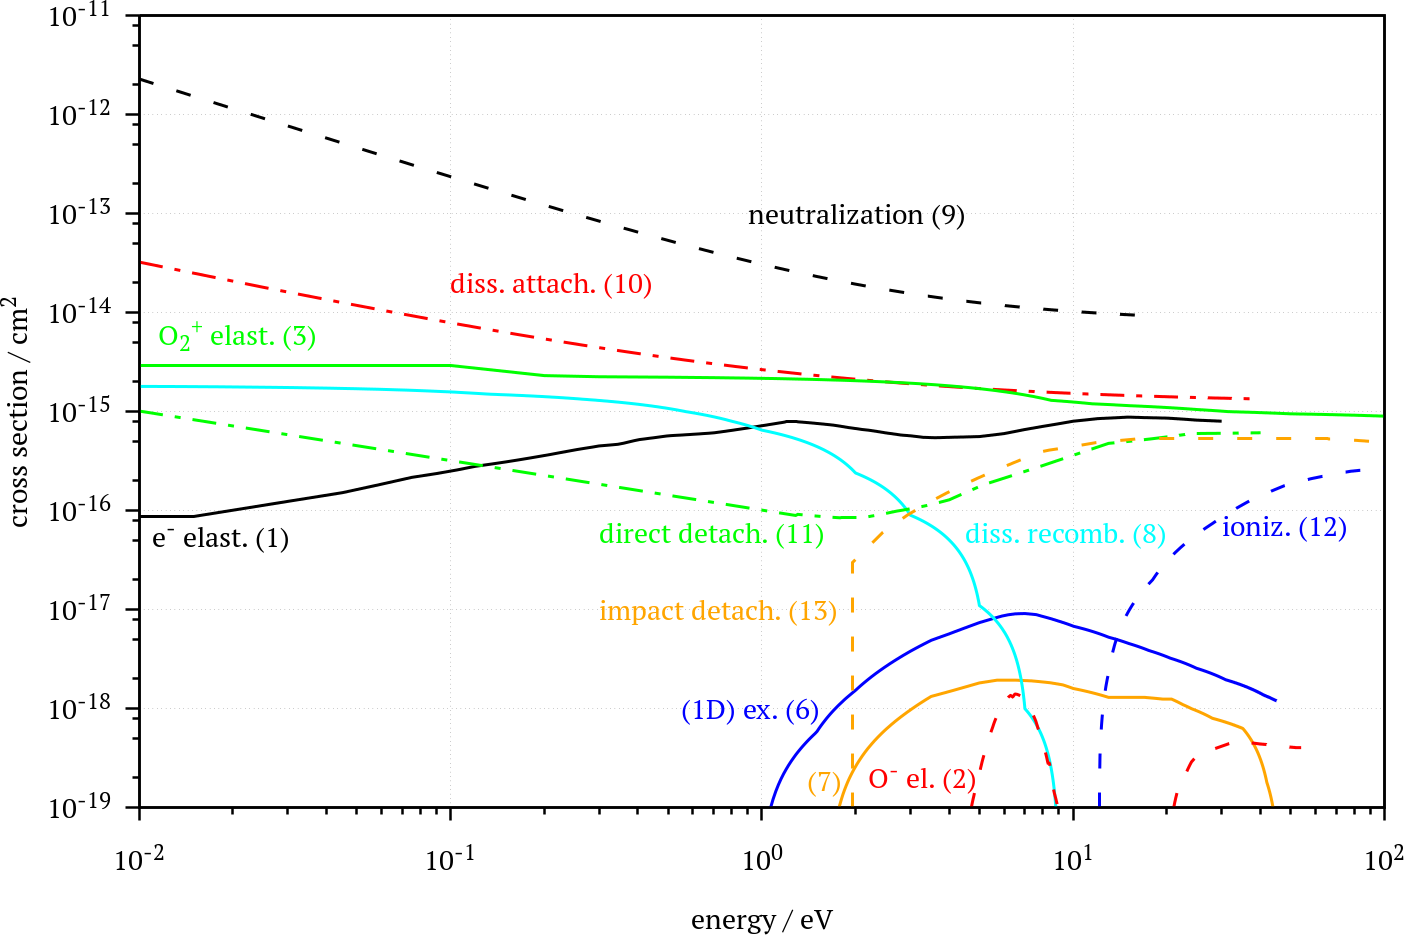
\includegraphics[width=1.0\textwidth]{figures/xsections.png}
				\caption{%
					Test.}%
				\label{fig:cross_sections}	
			\end{figure}	

%			
		\subsection{Anion Production}\label{sec:anionproduction}
%
